\section{Theorie}
\label{sec:Theorie}

\subsection{Bewegung von Elektronen in eniem elektrischen Leiter}

\noindent Elektronen in einem Atom befinden sich in verschiedenen Orbitalen, wobei aufgrund des Pauli-Prinzips nur maximal
zwei Elektronen mit unterschiedlichen Spinzuständen sich in einem Orbital befinden dürfen. Wenn diese sich in solch
einem Zustand befinden, dann kann das Energieniveau von den Elektronen kaum variieren, sodass es viel Energie
benötigt, um diese auf ein höheres Niveau zu bringen. \\

\noindent Elektronen in einem elektrischen Leiter bewegen sich durch Bänder. Diese Bänder sind überlappende Atomorbitale,
entlang welcher sich Elektronen bewegen. Hierbei bilden die Atome eine regelmäßige Kristallstruktur, was diese 
Überlappung ermöglicht. Um die notwendige Energie zu bekommen, um durch ein angelegtes elektrisches
Feld bewegt zu werden, müssen sich die Elektronen alleine in einem Orbital befinden. Ansonsten können sie nicht
ihr Orbital verlassen, da die notwendige Energie zu klein ist. \\

\noindent Desweiteren ist es möglich, dass in einem elektrischen Leiter die Bewegung der Löcher, die die Elektronen 
hinterlassen, überwiegt, was sich in dem Vorzeichen, der Ladungsdichte wiederspiegelt. Da solche Löcher als positiv e
Ladungen erscheinen, wird die Ladungsdichte auch positiv sein dann und andernfalls ist sie negativ.

\subsection{Der Halleffekt}

\noindent In einem Stromdurchflossenem Leiter, welcher von einem Magnetfeld durchflossen wird, werden die Elektronen senkrecht
zu der Stromrichtung und dem Magnetfeld abgelenkt. Dabei entsteht ein Ladungsüberschuss auf einer Seite, wodurch 
ein weiteres elektrisches Feld entsteht. Die dadurch entstandene Spannung ist dann messbar.
\begin{figure}[H]
    \centering
    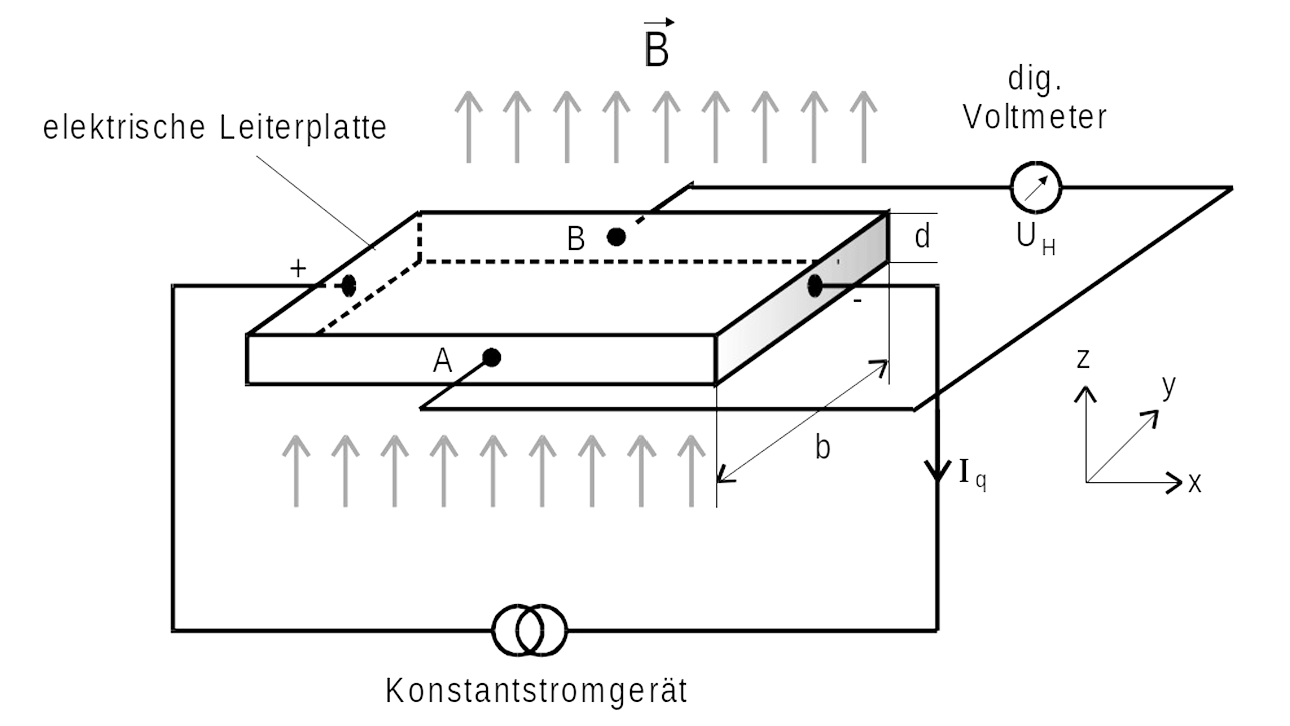
\includegraphics{Bilder/Halleffekt.png}
    \label{fig:Halleffekt}
\end{figure}

Die tatsächliche Hallspannung ergibt sich dann aus 
\begin{equation}
    U_H=\frac{1}{2}(U_+-U_-) \text{,}
    \label{eqn:stör}
\end{equation}
wobei $U_-$ die Messung ist, bei der der Strom umgepolt wird gegenüber der Messreihe $U_+$.

\subsection{Größen zur Beschreibung der Bewegung der Elektronen.}

\noindent Die Bewegung der Elektronen in einem Leiter kann über die Bewegung von Teilchen in einem idealen Gas betrachtet
werden, wobei das elektrische Feld eine bevorzugte Bewegungsrichtung vorgibt. Hierbei wird die Energieverteilung
der Elektronen durch eine Fermi-Dirac Verteilung
    \begin{equation}
         f(E)\symup{d}E=\frac{1}{e^(\frac{E-E_f}{kT})+1}\symup{d}E
         \label{eqn:fermidirac}
    \end{equation}   
\noindent beschrieben, wobei $E_f$ die Fermi-Energie ist, $k$ die Boltzmannkonstante und $T$ die Temparatur. Für die 
Fermi-Energie gilt dabei
\begin{equation}
    E_f=\frac{h^2}{2m_e}(\frac{3n}{8\pi})^(\frac{2}{3}) \text{,}
    \label{eqn:fermienergie}
\end{equation}
\noindent wobei $h$ das plancksche Wirkumsquantum ist, $m_e$ die Masse eines Elektrons und $n$ die Ladungsträgerdichte.
Diese Ladungsträgerdichte wird über den Halleffekt bestimmt.
\begin{equation}
    n=-\frac{BI_q}{dU_He_0}
    \label{eqn:ladungsdichte}
\end{equation}
\noindent $B$ ist ein von außen angelegtes Magnetfeld, $U_H$ die gemessene Hallspannung, $d$ die Dicke des Leiters und $e_0$
die Elementarladung.\\
\noindent Da die Elektronen als ein ideales Gas betrachtet werden, lässt sich auch eine mittlere Zeit $\bar{\tau}$ 
zwischen zwei Stössen bestimmen als
\begin{equation}
    \bar{\tau}=\frac{2m_e}{e_0^2n\rho}\text{,}
    \label{eqn:mittlere_Flugdauer}
\end{equation}
\noindent wobei $\rho$ der spezifische Widerstand des Materials ist. Der spezifische Widerstand ist eine Materialgröße,
welche einen Widerstand für die Elektronen durch defekte in der Kristallstruktur wiedergibt und wird über
\begin{equation}
    \rho=R\frac{A}{l}
    \label{eqn:spezifischer_widerstand}\text{,}
\end{equation}
\noindent mit der Querschnittsfläche $A$, der Leiterlänge $l$ und dem gemessenem Widerstand $R$, bestimmt.
Damit lässt sich die Anzahl der Ladungsträger pro Atom mit der molaren Masse $M$ und der Avogadrokonstante $N_A$ mit
\begin{equation}
    z=\frac{nM}{\rho N_A}
    \label{ladung_pro_atom}
\end{equation}
\noindent berechnen\\
\noindent Desweiteren lässt sich die mittlere Driftgeschwindigkeit mithilfe der Ladungsdichte und Stromdichte $j$ bestimmen.
\begin{equation}
    \bar{v}_d=-\frac{j}{ne_0}
    \label{eqn:drift}
\end{equation}
Zusätzlich zu der Driftgeschwindigkeit haben Elektronen noch eine Totalgeschwindigkeit
\begin{equation}
    |\bar{v}|=\bar{\tau}\sqrt{\frac{2E_f}{m_e}}\text{,} 
    \label{eqn:total}
\end{equation}
\noindent welche durch die thermische Bewegung der Teilchen entsteht. Damit lässt sich auch eine mittlere freie Weglänge $\bar{l}$
beschreiben, in der Elektronen ohne zusammenzustossen sich bewegen.
\begin{equation}
    \bar{l}=\bar{\tau}\sqrt{\frac{2E_f}{m_e}}
    \label{eqn:Weglänge}
\end{equation}
\noindent Zusätzlich lässt sich noch eine Beweglichkeit $\mu$ für die Elektronen definieren als
\begin{equation}
    \mu=\frac{e_0}{2m_e}\bar{\tau}\text{.}
    \label{eqn:Beweglichkeit}
\end{equation}

